\section{Background and Motivation}

\label{sec:overview}

In this section, we introduce the background knowledge of false sharing 
%of cache lines in the memory hierarchy 
and motivate the necessity of a lightweight tool to detect and quantify its impact in program execution. Finally, we overview \cheetah{} and propose our approaches.

\subsection{Background of False Sharing}
\label{sec:background}

In the multicore era, multithreading is the basic way to utilize underlying hardware cores by running different threads on different cores concurrently. When a thread modifies data of a cache line, the underlying cache coherence protocol (inside hardware) silently invalidates the duplicates of this cache line on other cores. This is to guarantee correct executions for true sharing instances like that shown in Figure~\ref{fig:tsinfs}. However, for false sharing cases (e.g. Figure~\ref{fig:fsinfs}), these invalidations are totally unnecessary when different threads are actually accessing different parts of the same line. Cache invalidations may force other cores to wait for reloading of data unnecessarily, wasting CPU time and precious memory bandwidth. A big amount of unnecessary cache invalidations can significantly impact the performance of software. As shown by the example shown in Figure~\ref{fig:penalty}, the false sharing problems can slowdown the performance of applications as much as an order of magnitude. The hardware trend, including adding more cores into the same machine, introducing the Non-Uniform-Memory-Access (NUMA) architecture, or increasing the size of a cache line, will further degrade the performance of false sharing problems, making the task of detecting more urgent. 
%Actually, as the evolution of the hardware, such as the uses of larger cache lines or the popularity of Non-Uniform-Memory-Access hardware, the false sharing problem can become increasingly serious. 

The performance of false sharing can be avoidable because of unnecessary cache invalidations, while true sharing can not. False sharing can be further categorized into inter-object and intra-object false sharing. When two different objects in the same cache line are accessed by different threads simultaneously, that is inter-object false sharing. Otherwise, it is intra-object false sharing.  %Thus, it is urgent to develop some tools and systems to tackle with this problem. 

\begin{figure}[htbp]
\centering
\subfigure[False sharing]{%
   \label{fig:fsinfs}
   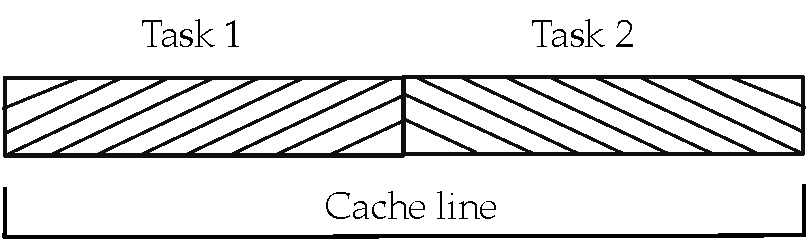
\includegraphics[width=2.4in]{figure/falsesharing}
}%
\hspace{30pt}
\subfigure[True sharing]{%
   \label{fig:tsinfs}
   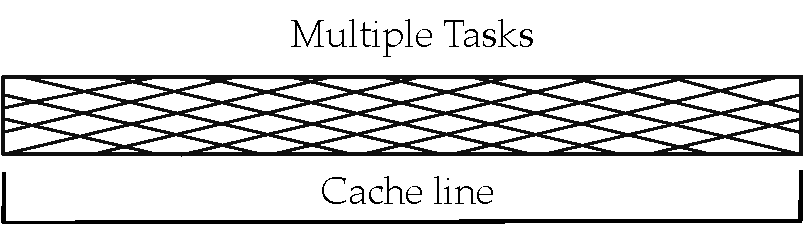
\includegraphics[width=2.4in]{figure/truesharing}
}%
\caption{False sharing (a) vs. true sharing (b). For false sharing, different tasks access different parts of the same cache line simultaneously. For true sharing, multiple tasks access the same part of a cache line.\label{fig:falsesharing}}
\end{figure}

Common programming practice can easily introduce false sharing. For an example shown in Figure~\ref{fig:penaltycode}, different threads access different words of the same global array, but involving in a big number of unnecessary cache invalidations. This problem is hard to find out manually by checking the results of executions.  

After the detection, there are several ways to fix them by preventing multiple threads from accessing the same cache line simultaneously. {\tt First},  we can pad useless words into a corresponding structure or class. {\tt Second}, we can assign the value of falsely-shared variable to a thread-local variable so that different threads may update their local variables, and commit those changes back to the shared variable in the end. {\tt Third},  some systems can isolate the execution of different threads, but with their own limitations on applications and the environment~\cite{Sheriff, OSdetection}. 
%However, Sheriff only works for multithreaded programs that are using the standard \pthreads{} library, without ad hoc synchronizations~\cite{Xiong:2010:AHS:1924943.1924955} and communication across the stack. 
Thus, mostly people are still using the first two approaches to fix false sharing problems by changing the code manually. For these approaches, programmers should have precise information about falsely-shared objects in order to fix them. \cheetah{} aims to provide precise information as much as possible, such as where are those falsely-shared objects, what is access pattern of memory accesses, and how much performance improvement after fixes. 


\sloppy
\subsection{Motivation of Efficient Memory Trace Collection}
Analyzing memory access patterns is an effective way to pinpoint false sharing. However, capturing memory accesses via software methods is costly, even with various sampling techniques~\cite{macpo,SLO2}. The overhead can be as high as 2-5$\times$, which is often not applicable to real applications working on large data sets and running in a highly threaded platform. Moreover, the high overhead leads to inaccurate measurement of program execution, which inconveniences the impact assessment of performance bottlenecks.

To address this issue, recent hardware performance monitoring units (PMU) support sampling memory accesses with extremely low overhead, less than 5\%. There are two typical sampling mechanisms in modern architectures: instruction-based sampling (IBS)~\cite{AMDIBS:07} supported in AMD Opteron processors and precise event-based sampling (PEBS) with load latency extension~\cite{IntelArch:PEBS:Sept09} in Intel Nehalem processors as well as their successors. Both IBS and PEBS can sparsely sample memory loads and stores at the same time. For each load sample, IBS and PEBS capture its effective address and the latency in CPU cycles from this sampled instruction issued to retired. For each store sample, IBS and PEBS capture its effective address only. Moreover, both IBS and PEBS record the precise instruction pointers of sampled memory accesses, which can be used to associate the analysis with program's source code. To make our analysis efficient, we build \Cheetah{} based on PMU sampling. 

 \subsection{Overview of Cheetah}

\begin{figure}[htbp]
\centering
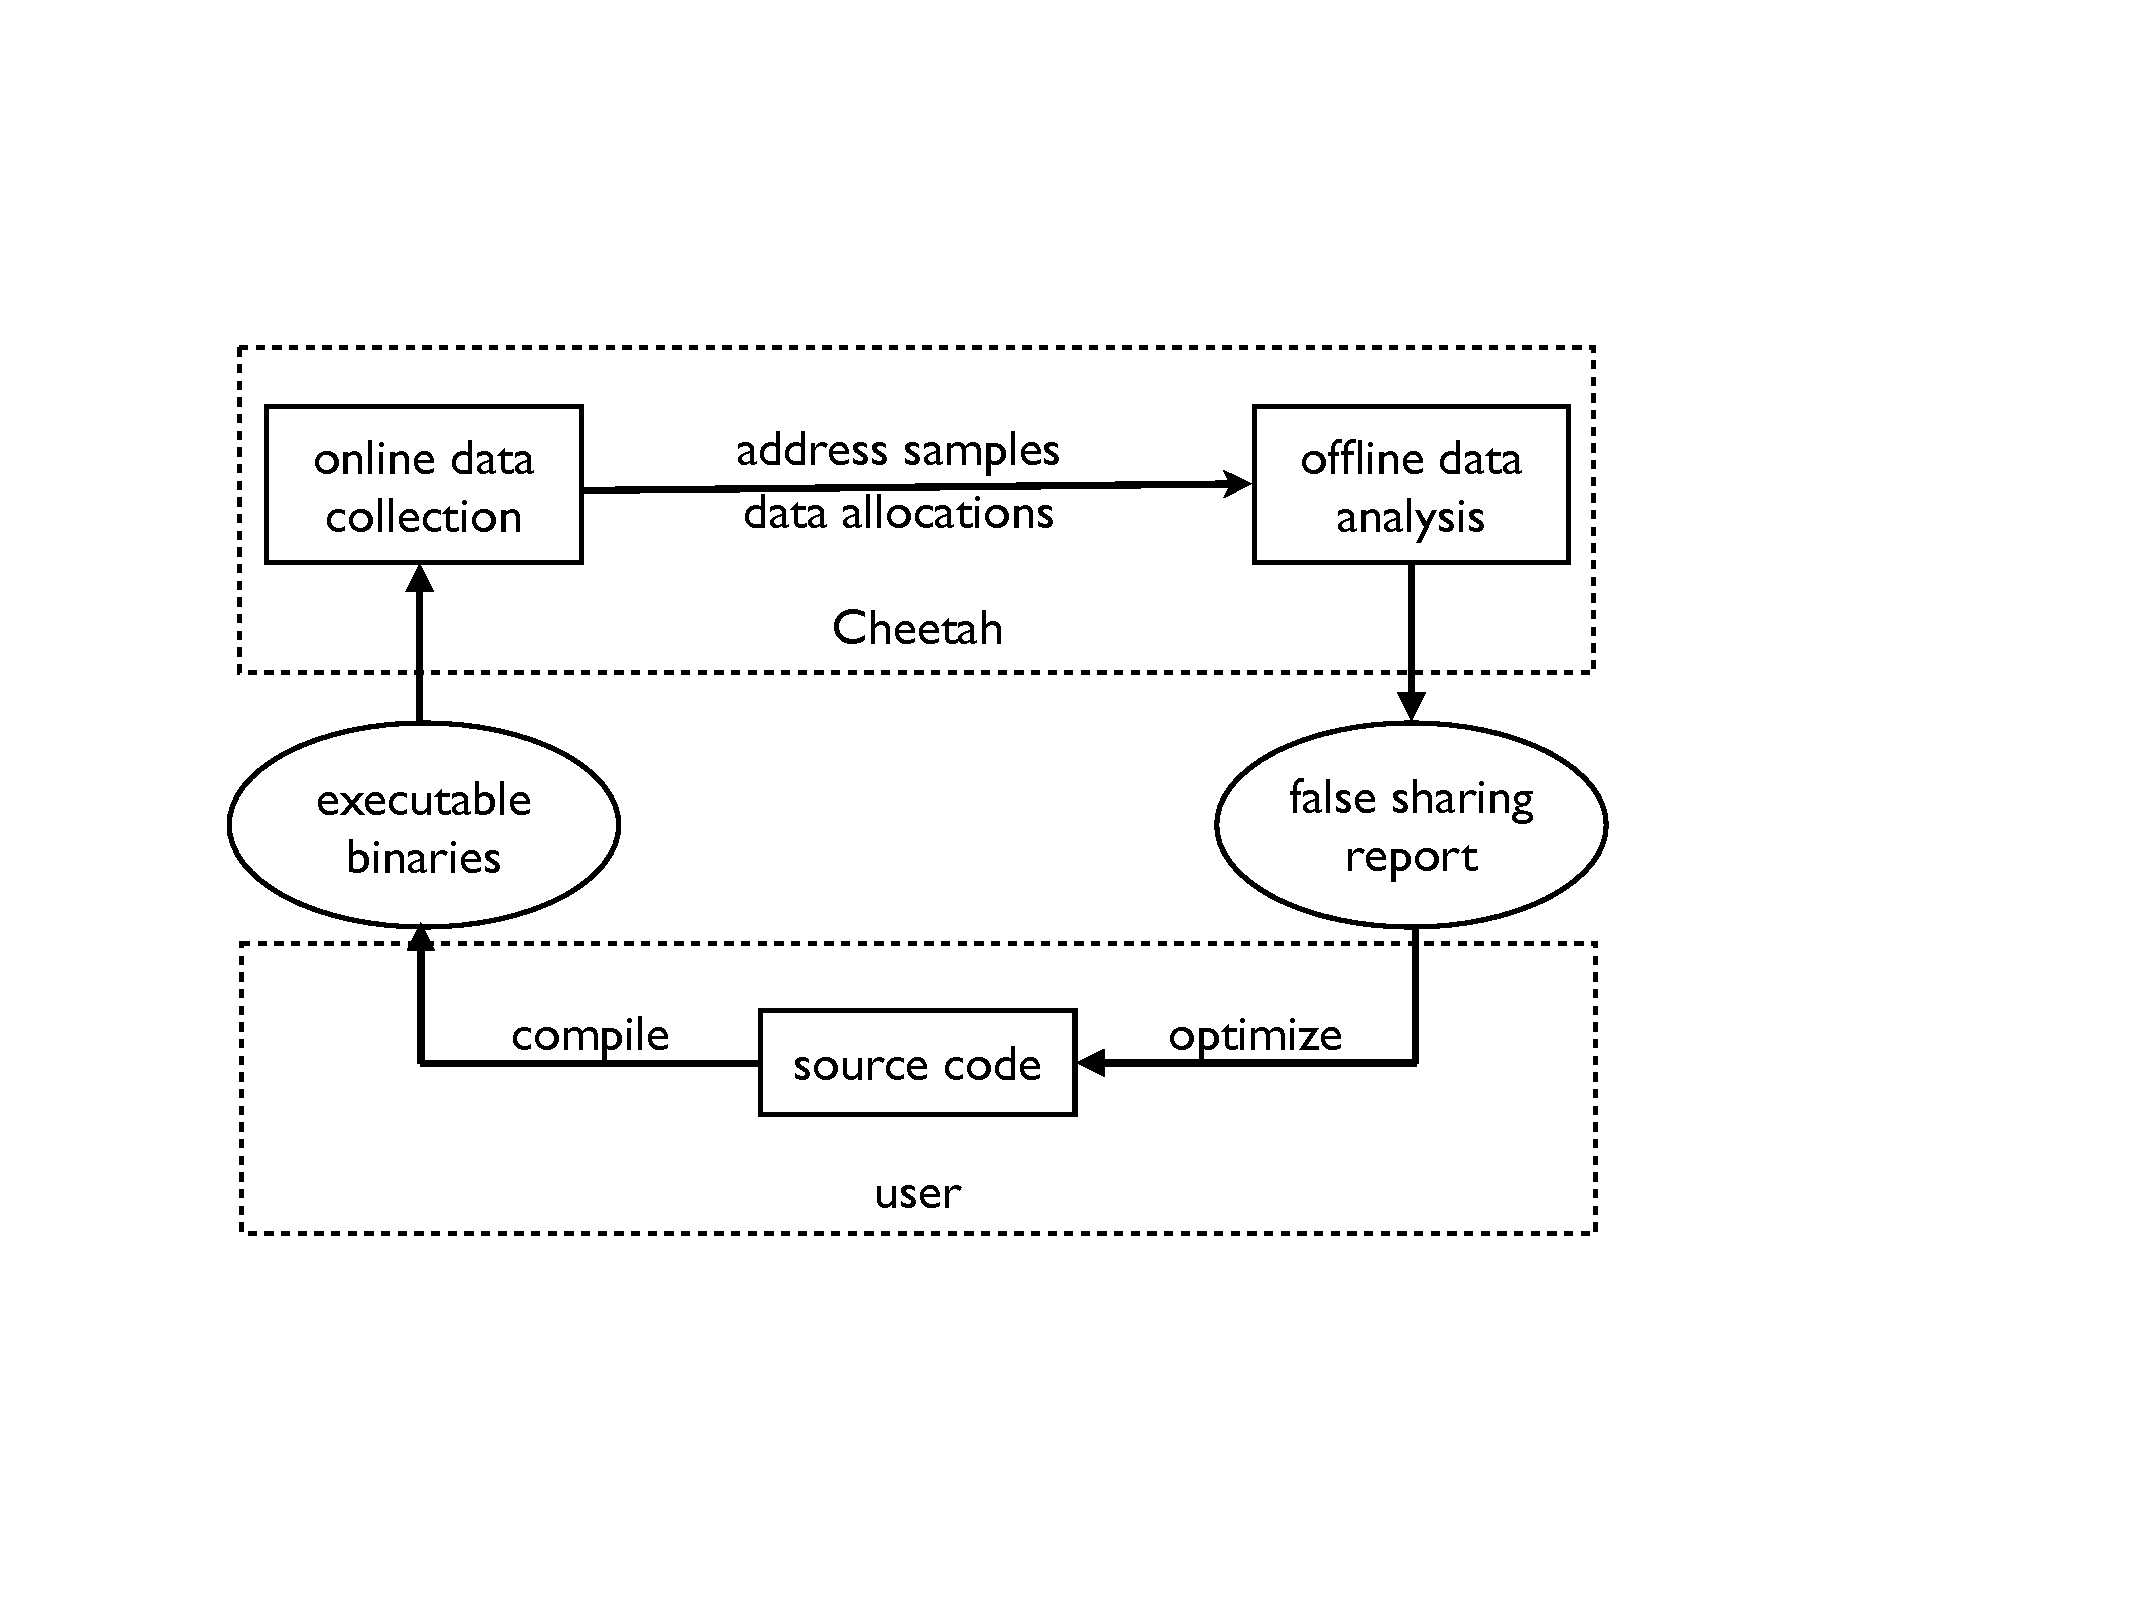
\includegraphics[width=\columnwidth]{figure/workflow}
\caption{The workflow of \cheetah{}}
\label{fig:workflow}
\end{figure}

\Cheetah{}, as shown in Figure~\ref{fig:workflow}, consists of two components: an online profiler and an offline analyzer. The online profiler leverages PMU to monitor program execution and the offline analyzer processes all performance data collected by the profiler. Finally, \cheetah{} generates a report to guidance programmers for code optimization. 
To distinguish \cheetah{} from existing tools, we claim that \cheetah{} can detect false sharing efficiently and effectively. For its efficiency, \cheetah{} incurs low runtime overhead, around 10\%, which is much lower than the state-of-the-art tool, such as Predator~\cite{Predator}. For its effectiveness, \cheetah{} precisely identifies false sharing, without reporting any true sharing. Moreover, it provides detailed optimization guidance, including source code information, data object information, and assessment of improvement potentials.

In the following two sections, we elaborate how \cheetah{} efficiently detects false sharing and assesses its impact to the whole program execution.


